%%%%%%%%%%%%%%%%%%%%%%%%%%%%%%%%%%%%%%%%%%%%%%%%%%%%%%%%%%%%%%%%%%%%%%%%%%%%%%%%%%%
%%%%%%%%%%%          Preamble
%%%%%%%%%%%%%%%%%%%%%%%%%%%%%%%%%%%%%%%%%%%%%%%%%%%%%%%%%%%%%%%%%%%%%%%%%%%%%%%%%%%%
\documentclass[9pt]{beamer}
\usepackage{setspace}
\usepackage{color}
\usepackage{amsmath,lmodern,amssymb,bm}
\usepackage{hyperref}
\usepackage{graphicx}
\usepackage{multirow}
\usepackage{subfig}
\usepackage[textfont={scriptsize}]{caption}
\usepackage{tikz}
\usetikzlibrary{fit,shapes.misc,arrows.meta,positioning}
\usepackage{pdflscape}
\usepackage{lscape}
\usepackage{enumerate}
\usepackage{epstopdf}
\usepackage{appendixnumberbeamer}
\usepackage{bigints}
\usepackage{booktabs}
\usepackage{color,soul}
\usepackage{grffile}
\usepackage{relsize}
\usepackage{mathtools}
\usepackage{tcolorbox}
 
% Colors
\definecolor{slideblue}{RGB}{0, 102, 153}
\setbeamercolor{frametitle}{fg=slideblue}
\setbeamercolor{title}{fg=slideblue}
\setbeamercolor{structure}{fg=slideblue}
\setbeamercolor{alerted text}{fg=red}
 
% Itemize markers
\setbeamertemplate{itemize items}[ball]
\setbeamertemplate{itemize subitem}[triangle]
\setbeamertemplate{itemize subsubitem}[triangle]
\beamertemplatenavigationsymbolsempty
\addtobeamertemplate{frametitle}{\vspace*{0.19cm}}{\vspace*{0cm}}
\setbeamertemplate{caption}{\raggedright\insertcaption\par}
\tcbset{colframe=white,colback=white,nobeforeafter}
 
% Tighter itemize spacing
\setlength{\leftmargini}{1em}
\setlength{\leftmarginii}{1em}
 
% Topline decorators
\newcounter{nodemarkers}
\newcommand{\toplinesmall}{%
  \tikz[remember picture,overlay] {%
    \draw[blue,thick] ([yshift=-.9cm, xshift=.9cm]current page.north west)
             -- ([yshift=-.9cm,xshift=3.6cm]current page.north west);}}
\newcommand{\toplinemedium}{%
  \tikz[remember picture,overlay] {%
    \draw[blue,thick] ([yshift=-.9cm, xshift=.9cm]current page.north west)
             -- ([yshift=-.9cm,xshift=6.2cm]current page.north west);}}
\newcommand{\toplinelarge}{%
  \tikz[remember picture,overlay] {%
    \draw[blue,thick] ([yshift=-.9cm, xshift=.9cm]current page.north west)
             -- ([yshift=-.9cm,xshift=8.9cm]current page.north west);}}
\newcommand{\toplinexlarge}{%
  \tikz[remember picture,overlay] {%
    \draw[blue,thick] ([yshift=-.9cm, xshift=.9cm]current page.north west)
             -- ([yshift=-.9cm,xshift=12cm]current page.north west);}}
 
% Footer
\setbeamertemplate{footline}{%
  \leavevmode%
  \hbox{%
    \begin{beamercolorbox}[wd=.33\paperwidth,ht=2.25ex,dp=1ex,left]{author in head/foot}%
      \usebeamerfont{author in head/foot}\hspace{1em}ECON712
    \end{beamercolorbox}%
    \begin{beamercolorbox}[wd=.34\paperwidth,ht=2.25ex,dp=1ex,center]{title in head/foot}%
      \usebeamerfont{title in head/foot}Winter 2026
    \end{beamercolorbox}%
    \begin{beamercolorbox}[wd=.33\paperwidth,ht=2.25ex,dp=1ex,right]{date in head/foot}%
      \usebeamerfont{date in head/foot}Lecture 15\hspace{1em}
      \insertframenumber{} / \inserttotalframenumber\hspace{1em}
    \end{beamercolorbox}}%
  \vskip0pt%
}
 
\newtheorem{proposition}[theorem]{Proposition}
 
\title{ECON 712: Applied Econometrics}
\author{Lecture 16: Differences-in-Differences}
\date{}
\AtBeginSection[]{
 \begin{frame}<beamer>
 \tableofcontents[currentsection]
 \end{frame}
}
 
%%%%%%%%%%%%%%%%%%%%%%%%%%%%%%%%%%%%%%%%%%%%%%%%%%%%%%%%%%%%%%%%%%%%%%%%%%%%%%%%%%%%
%%%%%%%%%%%          Document
%%%%%%%%%%%%%%%%%%%%%%%%%%%%%%%%%%%%%%%%%%%%%%%%%%%%%%%%%%%%%%%%%%%%%%%%%%%%%%%%%%%%
\begin{document}
\setbeamercovered{transparent}
 
\begin{frame}
\maketitle
\end{frame}
 

\begin{frame}
\frametitle{\: \: \: Introduction -- 2x2 DiD Setup}
\toplinelarge
\begin{itemize}
\item Suppose that we have a policy that is implemented at a point in time that affects only a group of individuals
\vspace{0.11in}
\item Also, assume that we have panel data on individuals observed before and after the policy is implemented as well as on individuals not affected by the treatment over the same period
\vspace{0.11in}
\item The goal is to estimate the average \textbf{causal effect} of the policy on the treated group
\end{itemize}
\end{frame}

\begin{frame}
\frametitle{\: \: \: Notation}
\toplinesmall
\begin{itemize}
\item Let $Y_{ist}$ denote the \textbf{outcome variable} for individual $i$, group $s$, and period $t$, where:
\vspace{0.08in}
\begin{itemize}
    \item $s = 1$: individual $i$ belongs to the \textbf{never-treated} group
    \vspace{0.05in}
    \item $s = 2$: individual $i$ belongs to the \textbf{eventually-treated} group
    \vspace{0.05in}
    \item $t = 1$: \textbf{pre-treatment} period
    \vspace{0.05in}
    \item $t = 2$: \textbf{post-treatment} period
\end{itemize}
\vspace{0.11in}
\item We use the \textbf{potential outcomes} notation $Y_{ist}(d)$, where $d$ denotes the treatment status:
\vspace{0.08in}
\begin{itemize}
    \item $Y_{ist}(0)$: outcome when individual $i$ is \textbf{not treated}
    \vspace{0.05in}
    \item $Y_{ist}(1)$: outcome when individual $i$ is \textbf{treated}
\end{itemize}
\vspace{0.11in}
\item The \textbf{observed} outcome is $Y_{ist} = Y_{ist}(0) + \big[Y_{ist}(1) - Y_{ist}(0)\big] \cdot \mathbf{1}[s=2, \, t=2]$
\end{itemize}
\end{frame}

%--------------------------------------------------------------
\begin{frame}
\frametitle{\: \: \: Average Treatment Effect on the Treated}
\toplinexlarge
\begin{itemize}
\item The object of interest is the \textbf{ATT} — the average causal effect of the policy on the treated group in the post-treatment period:
\[
\text{ATT} = E\!\left[Y_{ist}(1) - Y_{ist}(0) \mid s=2,\, t=2\right]
\]
\vspace{0.04in}
\item Since treatment is received by group $s=2$ at $t=2$, the first term is \textbf{observed}:
\[
E\!\left[Y_{ist}(1) \mid s=2,\, t=2\right] = E\!\left[Y_{ist} \mid s=2,\, t=2\right]
\]
\vspace{0.04in}
\item The second term is the \textbf{fundamental problem of causal inference} — the counterfactual outcome is never observed:
\[
E\!\left[Y_{ist}(0) \mid s=2,\, t=2\right] \quad \longleftarrow \text{unobservable}
\]
\vspace{0.04in}
\item We need an assumption to replace this counterfactual with observable quantities
\end{itemize}
\end{frame}

%--------------------------------------------------------------
\begin{frame}
\frametitle{\: \: \: Identification I: Cross-Sectional Comparison}
\toplinelarge
\begin{itemize}
\item \textbf{Assumption (Random Assignment):} Treatment is independent of potential outcomes,
so the never-treated group $s=1$ provides the counterfactual for $s=2$:
\[
E\!\left[Y_{ist}(0) \mid s=2,\, t=2\right] = E\!\left[Y_{ist}(0) \mid s=1,\, t=2\right] = E\!\left[Y_{ist} \mid s=1,\, t=2\right]
\]
\vspace{0.06in}
\item Under random assignment, the ATT is identified by a \textbf{cross-sectional comparison} of group means at $t=2$:
\[
\text{ATT} = E\!\left[Y_{ist} \mid s=2,\, t=2\right] - E\!\left[Y_{ist} \mid s=1,\, t=2\right]
\]
\vspace{0.06in}
\item \textbf{Limitation:} Random assignment to treatment is rarely available in observational settings; groups $s=1$ and $s=2$ typically differ in ways that also affect $Y_{ist}(0)$
\end{itemize}
\end{frame}

%--------------------------------------------------------------
\begin{frame}
\frametitle{\: \: \: Identification II: Before-After Comparison}
\toplinelarge
\begin{itemize}
\item \textbf{Assumption (No Time Trend):} The untreated potential outcome of the treated group does not change over time:
\[
E\!\left[Y_{ist}(0) \mid s=2,\, t=2\right] = E\!\left[Y_{ist}(0) \mid s=2,\, t=1\right] = E\!\left[Y_{ist} \mid s=2,\, t=1\right]
\]
\vspace{0.06in}
\item Under this assumption, the ATT is identified by a \textbf{before-after comparison} within the treated group:
\[
\text{ATT} = E\!\left[Y_{ist} \mid s=2,\, t=2\right] - E\!\left[Y_{ist} \mid s=2,\, t=1\right]
\]
\vspace{0.06in}
\item \textbf{Limitation:} Many outcomes evolve over time for reasons unrelated to the policy (macro shocks, trends); confounding time variation biases this estimator
\end{itemize}
\end{frame}

%--------------------------------------------------------------
\begin{frame}
\frametitle{\: \: \: Identification III: Parallel Trends}
\toplinelarge
\begin{itemize}
\item \textbf{Parallel Trends Assumption:} In the absence of treatment, both groups would have experienced the \emph{same} change in outcomes over time:
\[
\begin{aligned}
&E\!\left[Y_{ist}(0) \mid s=2,\, t=2\right] - E\!\left[Y_{ist}(0) \mid s=2,\, t=1\right] \\[4pt]
&\quad = E\!\left[Y_{ist}(0) \mid s=1,\, t=2\right] - E\!\left[Y_{ist}(0) \mid s=1,\, t=1\right]
\end{aligned}
\]
\vspace{0.04in}
\item Since $s=1$ is never treated and $s=2$ is untreated at $t=1$, the right-hand side is \textbf{fully observable}. Solving for the counterfactual:
\[
\begin{aligned}
E\!\left[Y_{ist}(0) \mid s=2,\, t=2\right]
  &= E\!\left[Y_{ist} \mid s=2,\, t=1\right] \\[4pt]
  &\quad + \underbrace{\left(E\!\left[Y_{ist} \mid s=1,\, t=2\right] - E\!\left[Y_{ist} \mid s=1,\, t=1\right]\right)}_{\text{common time trend}}
\end{aligned}
\]
\vspace{0.04in}
\item This pins down the \textbf{unobservable} counterfactual $E[Y_{ist}(0)\mid s=2,t=2]$ using only observed data
\end{itemize}
\end{frame}

%--------------------------------------------------------------
\begin{frame}
\frametitle{\: \: \: Identification III: The DiD Estimator}
\toplinelarge
\begin{itemize}
\item Substitute the counterfactual into the ATT:
\begin{align*}
\text{ATT} &= E\!\left[Y_{ist} \mid s=2,\, t=2\right] - E\!\left[Y_{ist}(0) \mid s=2,\, t=2\right] \\[4pt]
           &= E\!\left[Y_{ist} \mid s=2,\, t=2\right] - E\!\left[Y_{ist} \mid s=2,\, t=1\right] \\
           &\quad - \Big(E\!\left[Y_{ist} \mid s=1,\, t=2\right] - E\!\left[Y_{ist} \mid s=1,\, t=1\right]\Big)
\end{align*}
\vspace{0.04in}
\item Every term on the right is \textbf{observable}, so the ATT is identified:
\[
\begin{aligned}
\text{ATT} &= \underbrace{\Big(E\!\left[Y_{ist} \mid s=2,\, t=2\right] - E\!\left[Y_{ist} \mid s=2,\, t=1\right]\Big)}_{\Delta\,\text{treated}} \\[8pt]
           &\quad - \underbrace{\Big(E\!\left[Y_{ist} \mid s=1,\, t=2\right] - E\!\left[Y_{ist} \mid s=1,\, t=1\right]\Big)}_{\Delta\,\text{control}}
\end{aligned}
\]
\vspace{0.04in}
\item The DiD estimator \textbf{differences out} the common time trend, leaving only the causal effect of the policy on the treated group
\end{itemize}
\end{frame}


\begin{frame}
\frametitle{\: \: \: Example: Card and Krueger (1994)}
\toplinelarge
\begin{itemize}
\item The correctly specified OLS regression is an interaction with time and group fixed effects:
\[
Y_{ist} = \alpha + \gamma NJ_s + \lambda d_t + \delta(NJ \times d)_{st} + \varepsilon_{ist}
\]
\begin{itemize}
    \item $NJ_s$: dummy equal to 1 if observation is from New Jersey
    \item $d_t$: dummy equal to 1 if observation is from November (post period)
\end{itemize}
\vspace{0.08in}
\item This equation takes the following values:
\vspace{0.06in}

\begin{center}
\begin{tabular}{lcc}
\toprule
 & \textbf{Pre (Feb)} & \textbf{Post (Nov)} \\
\midrule
\textbf{PA (control)} & $\alpha$ & $\alpha + \lambda$ \\[4pt]
\textbf{NJ (treated)} & $\alpha + \gamma$ & $\alpha + \gamma + \lambda + \delta$ \\
\bottomrule
\end{tabular}
\end{center}
\vspace{0.08in}
\item The DiD estimator recovers $\delta$:
\[
\widehat{\delta} = (\overline{Y}_{NJ,Post} - \overline{Y}_{NJ,Pre}) - (\overline{Y}_{PA,Post} - \overline{Y}_{PA,Pre})
\]
\end{itemize}
\end{frame}

\begin{frame}
\frametitle{\: \: \: Example: Card and Krueger (1994)}
\toplinelarge
\begin{figure}
\centering
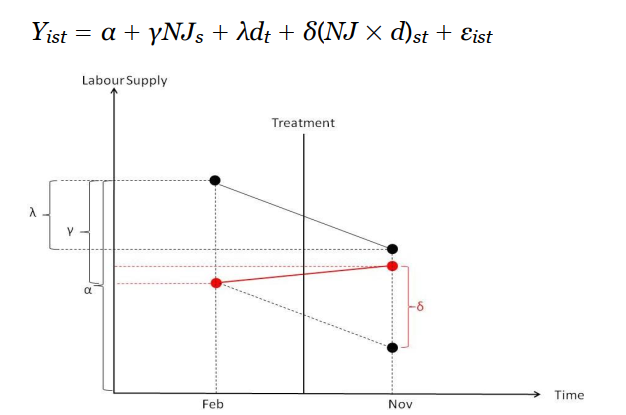
\includegraphics[scale=0.55]{card_Krueger2.png}
\end{figure}
\end{frame}

\begin{frame}
\frametitle{\: \: \: Example: Card and Krueger (1994)}
\toplinelarge
\begin{figure}
\centering
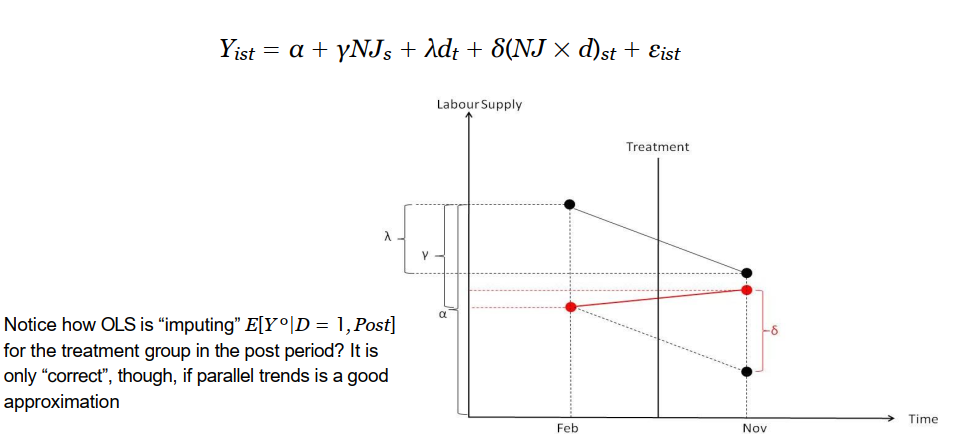
\includegraphics[scale=0.45]{card_Krueger3.png}
\end{figure}
\end{frame}

\begin{frame}
\frametitle{\: \: \: Card and Krueger (1994)-- what if parallel trends fail?}
\toplinexlarge
\begin{figure}
\centering
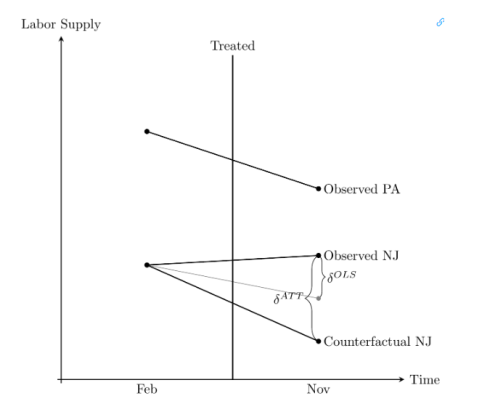
\includegraphics[scale=0.55]{card_Krueger4.png}
\end{figure}
\end{frame}




%--------------------------------------------------------------
\begin{frame}
\frametitle{\: \: \: Conclusion}
\toplinesmall
\begin{itemize}
\item DiD \textbf{relaxes} the two strong assumptions seen earlier:
\vspace{0.06in}
\begin{itemize}
    \item No need for \textbf{random assignment} across groups
    \vspace{0.04in}
    \item No need for \textbf{no time trends} within the treated group
\end{itemize}
\vspace{0.08in}
\item Instead, it imposes only \textbf{parallel trends}: treated and control groups would have followed the same trend absent treatment — a weaker condition
\vspace{0.08in}
\begin{itemize}
\item  Parallel trends can also fail if treatment is correlated with trends
\vspace{0.08in}
\item In such cases a \textbf{triple differences}, which extends the DiD along the same lines, might be able solve endogeneity issues
\end{itemize}
\vspace{0.08in}
\item   A critical practical issue arises when \textbf{treatment is assigned at the group level} (e.g.\ state, industry) but the regression is run at the individual level
\vspace{0.08in}
\begin{itemize}
\item In that case, all individuals within a group share the same treatment status, inducing \textbf{within-group correlation} in the residuals, so \textbf{cluster standard errors should be clustered at the level of treatment assignment} 
\vspace{0.08in}
\item \textbf{Card \& Krueger (1994)} is an example of this problem, with only two states, clustering is infeasible, which is a fundamental limitation of the design
\end{itemize}
\end{itemize}

\end{frame}

\end{document}




